% !TeX program = lualatex

\documentclass[12pt, a4paper]{article}

% --- Packages ---
\usepackage{enumitem}
\usepackage{fancyhdr}
\usepackage{fontspec}
\usepackage{geometry}
\usepackage{graphicx}
\usepackage[russian]{babel}
\usepackage{tikz}
\usepackage{titlesec}
\usepackage{hyperref}
\usepackage{xcolor}
\usepackage{wrapfig}

% --- Custom Colors ---
\definecolor{pagebg}{HTML}{F0D7B6}
\definecolor{bordercol}{HTML}{851F23}
\pagecolor{pagebg}

% --- Font ---
\setmainfont[
UprightFont = * Regular,
BoldFont    = * Bold,
ItalicFont  = * Italic,
BoldItalicFont = * BoldItalic,
]{Coats}

% --- Section Title Style ---
\newfontfamily\sectionfont{Coats Bold}\titleformat{\section}
{\sectionfont\fontsize{20pt}{24pt}\selectfont\bfseries\color{bordercol}}
{\thesection}{1em}{}

\titleformat{\subsection}
{\sectionfont\fontsize{15pt}{18pt}\selectfont\bfseries\color{bordercol}}
{\thesection}{1em}{}

% --- Page Border ---
\AddToHook{shipout/foreground}{
    \begin{tikzpicture}[remember picture,overlay]
        \draw[line width=1cm, bordercol]
            (current page.north west) rectangle (current page.south east);
    \end{tikzpicture}
}

% --- Page Setup ---
\geometry{margin=2.5cm}
\pagestyle{fancy}
\fancyhf{}
\fancyfoot[C]{\thepage}
\setlist{itemsep=0pt, topsep=8pt}

\sloppy

\begin{document}

% --- Title ---
\begin{center}
    {\fontspec{Segoe Script}
        \textcolor{bordercol}{\fontsize{36pt}{40pt}\selectfont Легенды Средневековья}
    }
\end{center}

\begin{wrapfigure}{r}{0.32\textwidth}
    \centering
    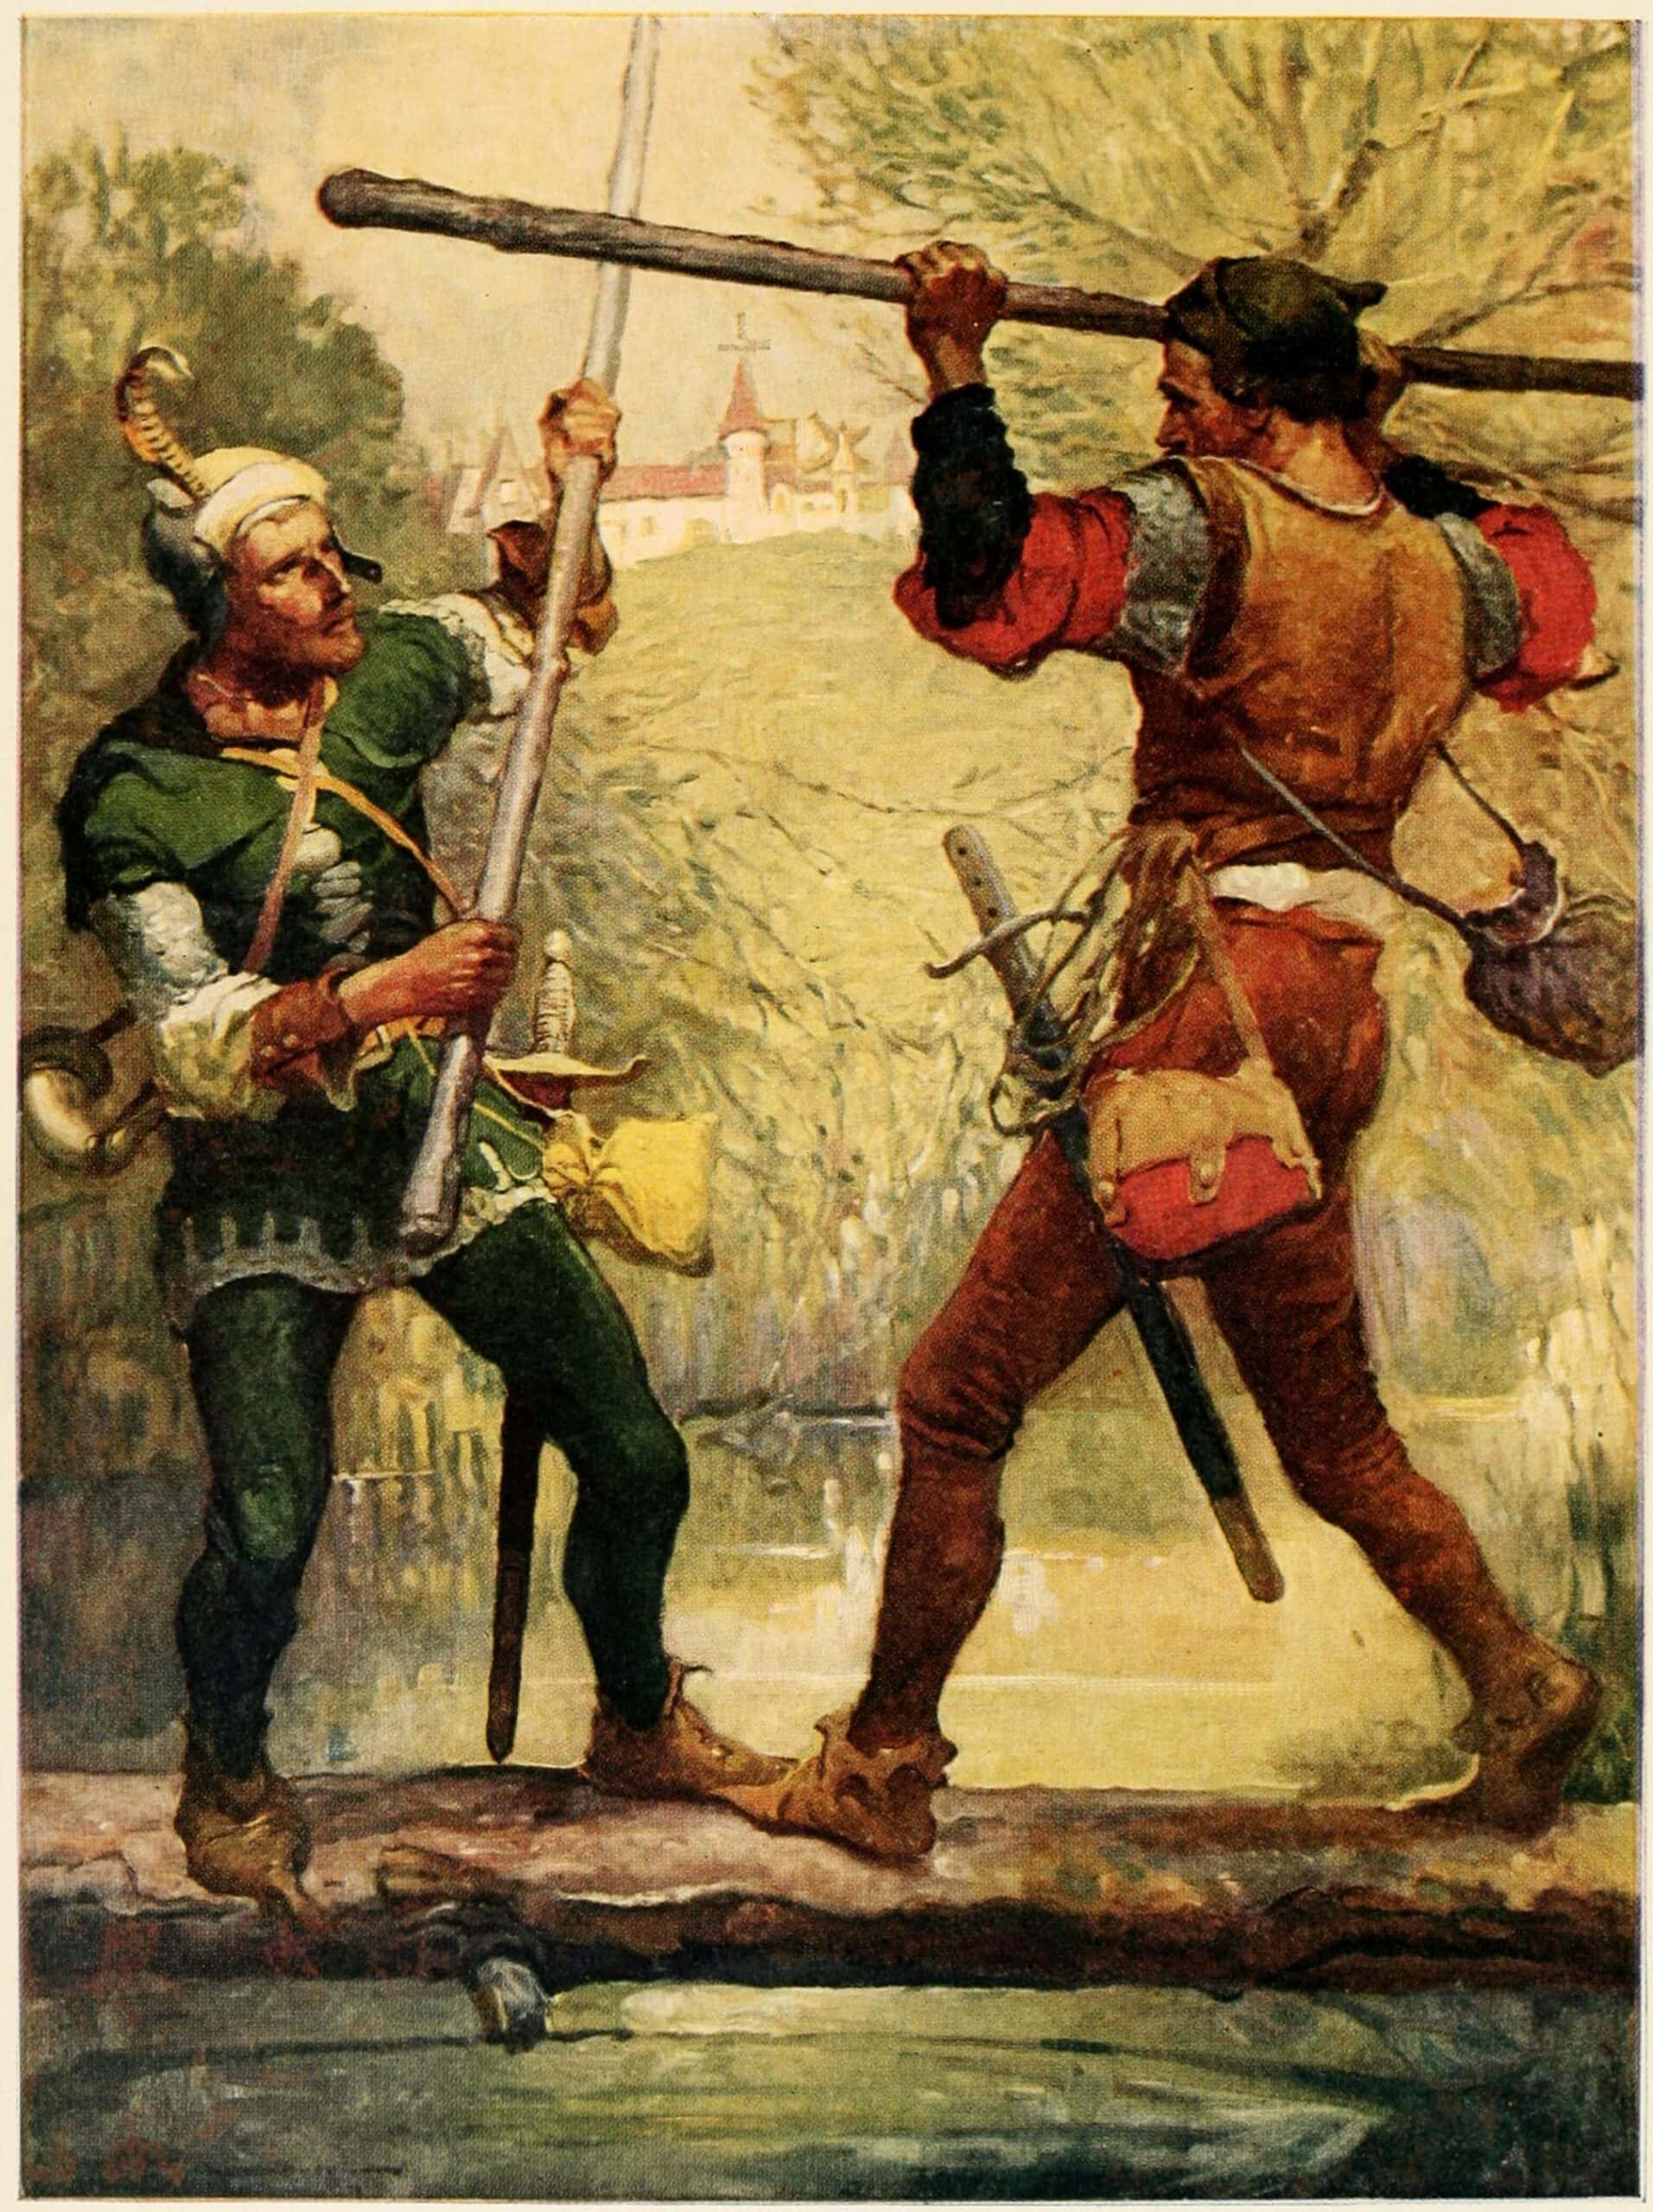
\includegraphics[width=0.30\textwidth]{Robin_Hood_and_Little_John-scaled.jpg}
\end{wrapfigure}

Глубоко в сердце Шервудского леса, среди вековых дубов, королевская
дорога между Лондоном и Йорком подвергалась набегам разбойников.
Богатые были вынуждены отдавать все, что имели, а простые люди
уходили свободными. Нуждающиеся получали одежду, еду и кров. Эта
банда разбойников, грабившая богатых и раздававшая добычу бедным,
противостояла тираническому игу несправедливых лордов и шерифов.
Кто был лидером этих борцов за социальную справедливость?

\textbf{Робин Гуд}, легендарный герой-разбойник из серии английских баллад, некоторые из которых датируются по крайней мере XIV веком. Робин Гуд был мятежником, и многие из самых ярких эпизодов в рассказах о нем показывают, как он и его товарищи грабят и убивают представителей власти, а добычу отдают бедным. Их самым частым врагом был шериф Ноттингема, местный представитель центральной власти (хотя внутренние свидетельства из ранних баллад ясно показывают, что действие происходило главным образом в южном Йоркшире, а не в Ноттингемшире). Среди других врагов были богатые церковные землевладельцы. Робин с уважением относился к женщинам, бедным и людям низкого социального положения. Во многом его восстание против власти было вызвано недовольством народа законами леса, ограничивавшими права на охоту. Ранние баллады, в особенности, раскрывают жестокость, которая была неотъемлемой частью средневековой жизни.

\newpage

\subsection*{Робин Гуд и Маленький Джон}

\begin{flushleft}

Как Робин и Джон повстречались в лесу, \linebreak
Поведаю вам без прикрас. \linebreak
Про это знакомство узнает потомство, \linebreak
И вас рассмешит мой рассказ. \linebreak

Маленький Джон был крепко сложен, \linebreak
Скорей дороден, чем худ. \linebreak
Семь футов росту детина имел, \linebreak
И весил кулак его пуд. \linebreak

Хоть маленьким люди прозвали его, \linebreak
Кому была жизнь дорога, \linebreak
От юного Джона не ждали разгона, \linebreak
А сами пускались в бега. \linebreak

В дубраве себя дожидаться велел \linebreak
Веселым стрелкам их вожак. \linebreak
– Пусть каждый стрелок услышит рожок, \linebreak
Если я попаду впросак. \linebreak

Две долгих недели не видели мы \linebreak
Ни дерзких забав, ни утех. \linebreak
От этакой скуки рассохнутся луки! \linebreak
Размяться мне, право, не грех! \linebreak

Беспечно отправился в путь Робин Гуд \linebreak
И видит – шагает чужак, \linebreak
Семи футов росту, по узкому мосту. \linebreak
Нельзя разминуться никак! \linebreak

Не тронутся с места ни тот ни другой; \linebreak
Обычай у них не таков. \linebreak
Никто на пядь не отступит вспять. \linebreak
Уперлись, как двое быков. \linebreak

Стрелу из колчана берет Робин Гуд \linebreak
С широким гусиным пером. \linebreak
– Тетиву натяну, и пойдешь ты ко дну, \linebreak
Когда не уступишь добром! \linebreak

У нас в Ноттингэме, – сказал Робин Гуд, \linebreak
Играть мы приучены так! \linebreak
– За эту игру я шкуру сдеру \linebreak
С тебя, – обещал чужак. \linebreak

\newpage

А Робин воскликнул: – Ты просто осёл! \linebreak
В надменное сердце твое, \linebreak
Прежде, чем глазом успеешь моргнуть, \linebreak
Вопьется стрелы острие. \linebreak

– Ты трус! – говорит незнакомец ему.– \linebreak
С чего поджимаешь ты хвост? \linebreak
При мне только сук, зачем же за лук \linebreak
Хвататься, ступив на мост? \linebreak

– Я слышал упрек, но им пренебрег. \linebreak
На землю сложив свой лук, \linebreak
Я разве не вправе себе в дубраве \linebreak
Выбрать увесистый сук? \linebreak

Торопится Робин из чащи лесной \linebreak
Покрепче дубину принесть: \linebreak
– Неужто не муж я и мне без оружья \linebreak
Нельзя отстоять свою честь? \linebreak

Сказал Робин Гуд: – Уговор будет прост: \linebreak
Кто с моста в проток угодил – \linebreak
Считай, что погиб, кормить ему рыб! \linebreak
А кто устоял – победил! \linebreak

Чужак согласился: – По мне – уговор! \linebreak
Не любишь ты обиняков. \linebreak
Я тоже не струшу, за милую душу \linebreak
Тебе надаю тумаков. \linebreak

Робин дубиной хватил чужака \linebreak
Так, что звякнул костяк. \linebreak
Сказал незнакомец: – Тебе возмещу \linebreak
С лихвой за этот пустяк! \linebreak

Мне страшно твоим должником умереть, \linebreak
Поверь моим словам! – \linebreak
Дубье, как цепы, что молотят снопы, \linebreak
Гуляло по их головам. \linebreak

Смельчак в это время дубиною в темя \linebreak
Нанес Робин Гуду удар. \linebreak
Как брызнет оттуда кровь Робин Гуда! \linebreak
Его даже бросило в жар! \linebreak

\newpage

Незлобен был Робин, однако способен \linebreak
Сто за сто воздать за зло. \linebreak
Росла свирепость ударов и крепость, \linebreak
А пуще всего – их число. \linebreak

Метнул незнакомец убийственный взор \linebreak
На Робина – и неспроста: \linebreak
Он с видом дерзким ударом зверским \linebreak
Противника сбросил с моста. \linebreak

– Ау, – вскричал со смехом чужак,– \linebreak
Откликнись, приятель, ты – где? \linebreak
– Клянусь, я тут! – отвечал Робин Гуд, \linebreak
Стуча зубами в воде. \linebreak

– Ты малый отважный, повадка твоя \linebreak
Мне, право, пришлась по нутру. \linebreak
Да будет известно, что выиграл честно \linebreak
Ты нынче нашу игру! \linebreak

Схватился герой за кустарник сырой \linebreak
И выбрался вон из воды. \linebreak
Не вплавь, так вброд, – говорит народ,– \linebreak
Робин Гуд ушел от беды. \linebreak

В рожок затрубив, пробудил Робин Гуд \linebreak
Дремавшее эхо долин. \linebreak
В одеждах зеленых – что твой изумруд – \linebreak
Стрелки собрались как один. \linebreak

– В чем дело, хозяин? – Вилл Статли спросил. \linebreak
С чего ты до нитки промок? \linebreak
– Промок я до нитки затем, что прыткий \linebreak
Юнец меня бросил в проток! \linebreak

Тут лучники, крепко схватив чужака, \linebreak
Кричат: – Не уйдешь невредим! \linebreak
Ты тоже в проток нырнешь, как нырок, \linebreak
А вынырнуть мы не дадим! \linebreak

– Моих сподручников, метких лучников – \linebreak
Семьдесят без одного! \linebreak
Ты парень отважный, – сказал Робин Гуд.– \linebreak
Не бойся теперь никого. \linebreak

\newpage

Зеленый наряд, приятный на взгляд, \linebreak
Придется тебе по плечу. \linebreak
По красному зверю тебя я сам \linebreak
Из лука стрелять научу. \linebreak

– Джон Маленький – люди прозвали меня. \linebreak
И, сколько осталось мне жить, \linebreak
Пусть проклят я буду, когда Робин Гуду \linebreak
Не стану верно служить! \linebreak

Сказал Вильям Статли: – Придется сменить \linebreak
Имя ему в добрый час! \linebreak
Я рад быть крестным, но день этот постным \linebreak
Не должен остаться для нас. \linebreak

На случай крещенья вкусней угощенья \linebreak
Никто не придумал досель, \linebreak
Чем жирная лань или нетель оленья \linebreak
И добрый разымчивый эль. \linebreak

Малыш миловидный – крепыш был завидный: \linebreak
Семь футов рост – не порок! \linebreak
А стан в перехвате был у дитяти, \linebreak
Что кряжистый дуб, широк. \linebreak

Вокруг младенца – новокрещенца – \linebreak
Лучники стали кольцом. \linebreak
Вилл Статли краткую речь произнес, \linebreak
Будучи крестным отцом: \linebreak

– Джон Маленький – имя ему не под стать. \linebreak
Но мы переставим слова, \linebreak
И Маленьким Джоном его будет звать \linebreak
Везде и повсюду молва. \linebreak

Тут клик веселый холмы и долы \linebreak
Потряс – и унесся ввысь. \linebreak
Обряд крестильный свершив, за обильный \linebreak
Пенистый эль принялись. \linebreak

В зеленый наряд, ласкающий взгляд, \linebreak
Дитя Робин Гуд одел \linebreak
Из собственных рук и дал ему лук \linebreak
С колчаном отточенных стрел. \linebreak

\newpage

– Нам злато жалеть нет нужды, заметь! \linebreak
Ты станешь отважным стрелком. \linebreak
Нам волей небес дан Шервудский лес \linebreak
И епископ с тугим кошельком. \linebreak

Как сквайры, как лорды, беспечны и горды \linebreak
Живем от забот вдали! \linebreak
Вина – что воды и вдоволь еды. \linebreak
Без фута земли – короли! \linebreak

Помедлив, багряное солнце сползло \linebreak
На лесом поросший склон. \linebreak
Шла пляска, покуда людей Робин Гуда \linebreak
Не принял в объятья сон. \linebreak

Их крестник был мужем, рослым и дюжим. \linebreak
Вдобавок на диво сложен, \linebreak
Храбр и не лжив, и, – сколько был жив,– \linebreak
Он звался Маленький Джон. \linebreak

\end{flushleft}


\newpage

\subsection*{Источники}

\begin{itemize}
    \item \href{https://www.nottinghamcastle.org.uk/the-legend-of-robin-hood/}{www.nottinghamcastle.org.uk/the-legend-of-robin-hood/} \\
    \item \href{https://www.historic-uk.com/HistoryUK/HistoryofEngland/Robin-Hood/}{www.historic-uk.com/HistoryUK/HistoryofEngland/Robin-Hood/} \\
    \item \href{https://www.britannica.com/topic/Robin-Hood}{www.britannica.com/topic/Robin-Hood}
\end{itemize}

\end{document}
